
\section{Brennstoffzelle}

\subsection*{Gefahren beim Umgang mit Sauerstoff und Wasserstoff}

Bevor nun auf die Funktionsweise eingegangen werden kann, muss erwähnt werden, wie gefährlich ein falscher Umgang mit Elementarem Sauerstoff und Wasserstoff sein kann.
Da elementarer Sauerstoff in unserer Atmosphäre vorkommt ist das freisetzen von $H_2$ an der Luft ausreichend um das gefährliche und hochexplosive Knallgas zu entwickeln. Ein bloßer Funke oder Reibung reicht nun aus um dieses Gas explosionsartig verbrennen zu lassen.
Hierbei entstehen Temperaturen bis zu 2000$^\circ$C.
Dies bedeutet auch, dass die Aufbewahrung kostspielig sein kann.
Aufgrund des sehr hohen Elektronegativitätenunterschiedes zwischen den beiden Elementen, sind sie im elementaren Zustand sehr reaktionsfreudig. Diese Potenzialdifferenz bestimt auch die maximal mögliche Spannung von ca. $\SI{1,3}{\volt}$.
Praktische gemessene Werte befinden sich jedoch aufgrund Verluste im Aufbau, bei einem maximalen Wirkungsgrad von 60\%, unter einem Volt.
Verluste können vom Brennstoff, von der Qualität der Zelle und von der Temperatur abhängen.
Zur erhöhung der gewonnen Spannung lassen sich mehrere Brenntstoffzellen aneinander ketten.
Aufgrund der Tatsache, dass Wasserstoff leicht herzustellen ist, ist die Brennstoffzelle dennoch ein wichtiges Forschungsgebiet.
Sie kann helfen, den Bedarf von tragbaren Energiequellen zu stillen, zudem sie ohne Risiken für Umwelt funktioniert.
%Wasserstoff und Sauerstoff ergeben im richtigen Stoffmengenverhältnis das hochexplosive Gasgemisch Knallgas.Bei Kontakt mit Funken kommt es zu einer denotationsartigen Verbrennung.

\subsection*{Maximalspannung einer Solar-/Brennstoffzelle}
Die maximale Spannung einer Solarzelle ist vorrangig durch das Halbleitermaterial begrenzt. Bei der Brennstoffzelle gibt das chemische Potential zwischen Wasserstoff und Sauerstoff die Spannung vor.

\subsection*{Funktionsprinzip einer Brennstoffzelle}

Im Folgenden soll auf die Funktionsweise der Brennstoffzelle eingegangen werden. 
Entgegen der Elektrolyse von Wasser sollen nun die Elementaren Moleküle, $H_2$ und $O_2$, zu elektrischer Energie zurückreagieren.
Stark vereinfacht lässt sich die Brennstoffzelle als Galvanisches Element darstellen, also, Anode und Kathode getrennt von einer semipermeablen Membran.
Die trennende Membranschicht benötigt also die Eigenschaft $H^+$ Ionen passieren lassen zu können.
Durch das Ionomer, ein protonendurchlässiges Polymer, können nur Protonen, nicht jedoch Stoffe wie Sauerstoff oder Wasserstoff, passieren.
Hierzu verwendet man zum Beispiel, ähnlich zu den klassischen Galvanischen Zellen, Laugen oder Säuren als flüssige Membran und Keramiken als Feste Membranschichten.
Durch ihre Eigenschaft hat sie auch den Namen PEM-Membran ("Proton Exchange Membrane") bekommen.
\begin{figure}
	\centering
	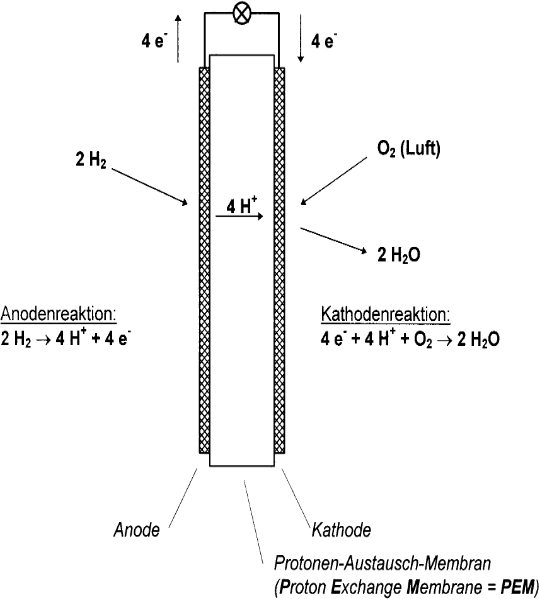
\includegraphics[width=0.6\textwidth]{Abb/brennstoffzelle.png}
	\caption{Funktionsweise der Brennstoffzelle}
	\label{zelle}
\end{figure}
Abbildung \ref{zelle} verdeutlicht Aufbau und Funktionsweise.

Entscheidend ist die Reaktionsgleichung, sie sorgt für frei Elektronen, die nun für den elektrischen Strom genutzt werden können.
Anode:
$2 H_2 \rightarrow 4 H^+ + 4e^-$
Kathode:
$O_2 + 4 H^+ + 4 e^- \rightarrow 2 H_2O$
Gesamtgleichung:
$2 H_2 + O_2 \rightarrow 2 H_2O$

An der Anode docken $H_2$ Moleküle an, geben ihr Elektron an einen Leiter ab und wandern als Protonen durch die Membran zum Sauerstoff.
An der Kathode Reagieren dann $2 H_2$ und $O_2$ zu $2 H_2O$.


Die maximale Spannung einer Solarzelle ist vorrangig durch das Halbleitermaterial begrenzt. Bei der Brennstoffzelle gibt das chemische Potential zwischen Wasserstoff und Sauerstoff die Spannung vor.
